\documentclass{dhbenelux}

\usepackage{booktabs} % for toprule, midrule, bottomrule in tables
\usepackage{authblk} % for multiple authors and affiliations
\usepackage{graphicx} % to inlcude graphics with \includegraphics
\usepackage{courier}
\usepackage{array}
\usepackage{listings}
\usepackage{tabularx}
\usepackage{longtable} % For long tables (if needed)
\usepackage{adjustbox}
\usepackage{amsmath}
\usepackage{algorithm}
\usepackage{algpseudocode}




\author[1]{Anirudh Dambal}
\author[1]{Harish Patil}
\author[1]{Pavan Bhakta}
\author[1]{Anusha Adarakatti}

\affil{School of Computer Science and Engineering,
KLE Technological University, Hubballi, Karnataka, India, 580031}

\title{Code to Code Conversion from Java to Python
Using T5-Small}

\begin{document}

\maketitle

\begin{abstract}
    \noindent {This paper introduces a new method of code-to-code translation from Java to Python using the T5-small transformer model, based on a custom-generated dataset. Previous works often depend on language-specific libraries or attributes; however, our dataset prohibits such inbuilt functionalities to promote the creation of fully translatable, algorithmically pure code. The dataset was generated with the help of the Gemini model, where sample text was initially translated into pseudocode, then coded into both Java and Python without language-specific shortcuts. This dataset was next used to train a T5-small model, which learned generalized patterns and structures for code translation. Evaluation results indicate the potential for using the T5-small model to translate Java code into Python with good accuracy in producing semantically equivalent and syntactically correct code. Our approach opens a promising direction for tool-assisted cross-language code translation, with significant implications for software development, maintenance, and education in multilingual coding environments.
}
\end{abstract}

\begin{keywords}
    {Transpilation, Encoder-Decoder Architecture, Multilingual Code Translation, Custom Dataset Generation, Pseudocode-Based Training, Gemini API, Cross-Language Programming}
\end{keywords}
\section{Introduction}

Code-to-code translation addresses real-world challenges such as adapting legacy systems to new technologies, improving code maintainability, and increasing cross-language collaboration. For example, businesses transitioning from Java to Python may aim to leverage Python’s rich data science libraries without discarding years of development in Java. This requires reliable methods to convert existing codebases accurately while preserving their original logic and functionality.

Domain-Specific Languages (DSLs) like Spark, NumPy, TACO, and P4 have changed the face of modern software development process by providing optimizations and abstractions tailored to specific applications. They improve code clarity, usability, and performance. However, they often require rewriting legacy code-a very tedious and error-prone process that risks changing the original behavior. Transpilation, or translating code between high-level languages, remains a significant challenge.

Recent advancements in Large Language Models (LLMs), such as BERT, GPT-3, and T5, have been promising in the automation of programming tasks like code generation and repair. Still, reliable code translation remains a challenge because most models lack robustness and correctness guarantees. In addition, formal verification tools depend on niche languages like SMT-LIB and Dafny, which are underrepresented in LLM training datasets, thus limiting their practical application.

The core challenge lies in translating code between high-level languages with distinct syntax and semantics, such as Java and Python. Current transpilation methods demand manual effort and expertise, which reduces efficiency and increases the risk of errors. While LLMs offer potential solutions, existing models often fail to address these limitations in real-world scenarios.

The main goals of this paper are to curate a dataset of paired Java and Python programs for training. The study attempts to determine the efficacy of the T5 model in automating the translation of Java to Python code and addresses the practical challenges encountered by developers, such as syntactic and semantic differences between the two languages.

The rest of the paper is organized as follows: Section 2 reviews related work, focusing on advancements in machine learning techniques for programming tasks. Section 3 outlines the proposed methodology, including dataset preparation and model training. Section 4 presents experimental results, analyzing the T5 model's performance in code translation. Section 5 discusses key findings and future research directions. Finally, Section 6 concludes with insights into the study's contributions.



\section{Related Work}

The application of machine learning models to programming tasks has seen significant advancements in recent years. Early research focused on representing code for machine learning purposes, leveraging hierarchical structures such as Abstract Syntax Trees (ASTs). Researchers like Tai et al. (2015) introduced Tree-LSTM models, which encode tree structures by processing nodes recursively, starting from the leaves. Mathematically, Tree-LSTMs extend the standard LSTM to handle tree-structured data by defining cell states and hidden states for each node \( i \) based on its child nodes \( C(i) \):
\[
h_i, c_i = \text{TreeLSTM}(x_i, \{h_{j}, c_{j} \,|\, j \in C(i)\}).
\]
This innovation laid the groundwork for program analysis and transformation. A schematic representation of the Tree-LSTM architecture can be illustrated in Figure~\ref{fig:tree-lstm}.

\begin{figure}[h]
    \centering
    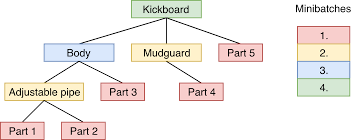
\includegraphics[width=0.8\textwidth]{Images/1.png}} % Replace with actual Tree-LSTM flowchart
    \caption{Tree-LSTM Architecture for AST Processing}
    \label{fig:tree-lstm}
\end{figure}

Chen et al. (2018) extended this approach by proposing a tree-to-tree encoder-decoder framework tailored specifically for code. This framework enabled structured transformations between different tree representations, such as converting an AST of one language into another. The encoder mapped the source tree \( T_s \) into a latent representation \( z \), and the decoder reconstructed the target tree \( T_t \). Formally:
\[
z = f_{\text{encoder}}(T_s), \quad T_t = f_{\text{decoder}}(z).
\]
Drissi et al. (2018) refined these ideas further by introducing the Left-Child Right-Sibling (LCRS) representation, simplifying tree encoding by reducing tree structures into binary trees, which proved effective for program translation tasks.

\begin{figure}[h]
    \centering
    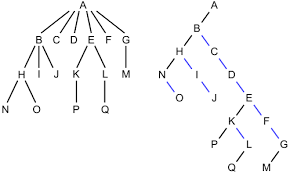
\includegraphics[width=0.8\textwidth]{Images/2.png}} % Replace with actual flowchart for tree-to-tree model
    \caption{Tree-to-Tree Encoder-Decoder Framework for Code Transformation}
    \label{fig:tree-encoder-decoder}
\end{figure}

The advent of neural machine translation (NMT) frameworks inspired new applications beyond natural language. Tufano et al. (2018) explored automated bug fixing by applying NMT to software maintenance tasks. They mined GitHub for bug-fix commits and abstracted code changes into generalizable patterns. Using tools like GumTree for edit tracking, they trained models capable of generating patches resembling developer edits. The loss function used to train the model, minimizing syntactic and semantic differences between generated and ground truth patches, is expressed as:
\[
\mathcal{L} = \sum_{i=1}^N \text{CrossEntropy}(\hat{y}_i, y_i),
\]
where \( \hat{y}_i \) is the predicted token and \( y_i \) is the actual token. Their approach achieved high syntactic correctness and underscored the utility of NMT in learning transformations at the AST level.

\begin{figure}[h]
    \centering
    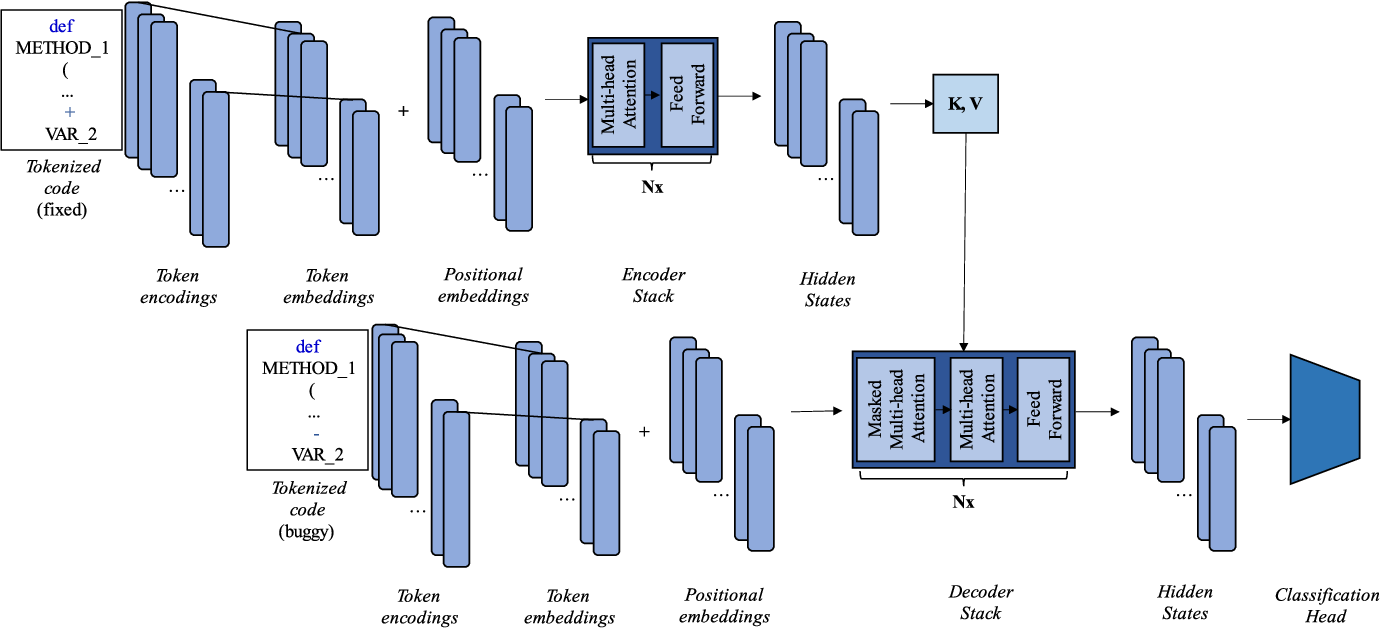
\includegraphics[width=0.8\textwidth]{Images/3.png}} % Replace with NMT bug fixing diagram
    \caption{Neural Machine Translation for Automated Bug Fixing}
    \label{fig:nmt-bug-fixing}
\end{figure}

Lachaux et al. (2020) introduced TransCoder, a system for translating functions between programming languages without requiring parallel training data. By leveraging monolingual source code and unsupervised learning techniques, TransCoder captured language-specific patterns. The objective was to minimize a combined reconstruction and translation loss:
\[
\mathcal{L} = \mathcal{L}_{\text{reconstruction}} + \mathcal{L}_{\text{translation}},
\]
where \( \mathcal{L}_{\text{reconstruction}} \) ensures that monolingual data reconstructs correctly, and \( \mathcal{L}_{\text{translation}} \) aligns the latent spaces of source and target languages. TransCoder outperformed rule-based systems, showcasing robust language-agnostic representations.

\begin{figure}[h]
    \centering
    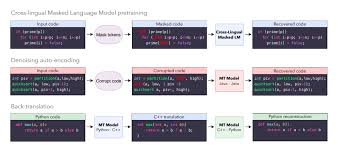
\includegraphics[width=0.8\textwidth]{Images/4.jpg}
    \caption{TransCoder Framework for Unsupervised Code Translation}
    \label{fig:transcoder}
\end{figure}

Katz et al. (2019) addressed decompilation, converting low-level code to high-level programming languages. Traditional decompilers relied on expert-crafted rules, but Katz et al. proposed a neural model to reverse compiler processes. Their NMT-based framework achieved high success rates in translating LLVM IR and x86 assembly back to source code, with substantial improvements over rule-based systems. 

More recently, Armengol-Estapé et al. (2021) explored transformer models for compilation tasks, marking a shift towards leveraging large pre-trained models. Transformers, with their self-attention mechanisms, allowed efficient modeling of long-range dependencies in code. The attention mechanism is expressed as:
\[
\text{Attention}(Q, K, V) = \text{softmax}\left(\frac{QK^\top}{\sqrt{d_k}}\right)V,
\]
where \( Q \), \( K \), and \( V \) are query, key, and value matrices, and \( d_k \) is the dimensionality of the keys. These models opened new possibilities for tasks like code generation, translation, and repair.

\begin{figure}[h]
    \centering
    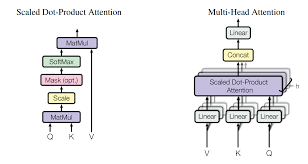
\includegraphics[width=0.8\textwidth]{Images/5.png}} % Replace with transformer-based model diagram
    \caption{Transformer Model for Compilation Tasks}
    \label{fig:transformer-code}
\end{figure}

These advancements collectively illustrate the evolution of machine learning techniques for programming tasks. From tree-based models to NMT and transformers, each step has contributed to a deeper understanding of how programs can be represented, translated, and optimized, forming the foundation for the methods explored in this work.


\section{Proposed Work}

This work presents a transpilation framework for automatic translation between high-level programming languages, namely Java and Python, using a fine-tuned T5-small model. The framework employs the encoder-decoder architecture of T5-small to capture syntactic and semantic differences between these languages. The implementation focuses on training and inference, achieving a robust pipeline for translating Java code into Python.

\subsection{Dataset preparation}
    The dataset was generated with the help of the Gemini model, where sample text was initially translated into pseudocode, then coded into both Java and Python without language-specific shortcuts.
\begin{enumerate}
    Dataset preparation involves generating pseudocode-based paired code snippets. 
    \begin{figure}[h!]
\centering
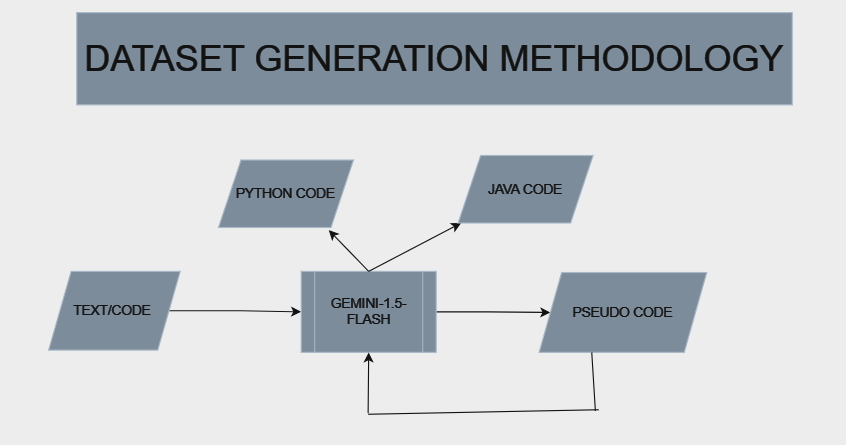
\includegraphics[width=0.7\textwidth]{dataset_methodology.png} % Replace with actual flowchart file
\caption{Dataset Preparation Methodology}
\end{figure}
\end{enumerate}
\subsubsection{Algorithms and Processes}

\begin{algorithm}
\caption{Automated Generation of Code Implementations from Pseudocode}
\label{alg:code_generation}
\begin{algorithmic}[1]
\Require 
\begin{itemize}
    \item A dataset of pseudocode samples with corresponding Java and/or Python code (if available).
    \item A generative AI model pre-trained on natural language and code (e.g., Gemini-1.5).
\end{itemize}
\Ensure 
\begin{itemize}
    \item A comprehensive dataset containing pseudocode and its generated Java and Python implementations.
    \item Evaluation-ready outputs for benchmarking generative model performance.
\end{itemize}

\State \textbf{Step 1: Data Preparation}
\State Initialize a structured dataset (\texttt{Dataset}) to store pseudocode and corresponding code implementations.
\State Save the dataset to a file format suitable for downstream evaluation (e.g., \texttt{PreparedDataset.csv}).

\State \textbf{Step 2: Model Configuration}
\State Configure a pre-trained generative AI model for code generation, specifying the appropriate API key or model parameters.

\State \textbf{Step 3: Pseudocode-to-Code Translation}
\For{each pseudocode sample in the dataset}
    \State \textbf{Input:} Provide the pseudocode as input to the generative model.
    \State \textbf{Prompt Engineering:} Design prompts to elicit:
    \begin{itemize}
        \item \textbf{Python Code Generation:} Generate Python code corresponding to the pseudocode.
        \item \textbf{Java Code Generation:} Generate Java code corresponding to the pseudocode.
    \end{itemize}
    \State \textbf{Output:} Store the generated Java and Python code in the dataset.
\EndFor

\State \textbf{Step 4: Dataset Augmentation}
\State Expand the dataset by integrating additional samples, if available, from a secondary pseudocode dataset.

\State \textbf{Step 5: Model Evaluation (Optional)}
\State Evaluate the generative AI model's output using code correctness and functional equivalence metrics, comparing with ground truth implementations if available.

\State \textbf{Step 6: Dataset Finalization}
\State Save the augmented dataset, including all pseudocode and generated implementations, to facilitate reproducibility and further research.

\end{algorithmic}
\end{algorithm}

\begin{algorithm}
\caption{Training and Evaluation of a Code Translation Model}
\label{alg:code_translation}
\begin{algorithmic}[1]
\Require 
\begin{itemize}
    \item A pre-trained T5 transformer model.
    \item A parallel dataset of Java and Python code samples.
\end{itemize}
\Ensure A fine-tuned model capable of translating Java code to Python.

\State \textbf{Step 1: Model Initialization}
\State Load a pre-trained T5 transformer as the base translation model.
\State Configure the model for the specified hardware (e.g., GPU or CPU).

\State \textbf{Step 2: Data Preparation}
\State Retrieve a parallel dataset containing Java code and corresponding Python translations.
\State Split the dataset into training and validation subsets (e.g., 75\% for training, 25\% for validation).

\State \textbf{Step 3: Model Fine-Tuning}
\State Fine-tune the T5 transformer using the training dataset:
\begin{itemize}
    \item Define the loss function to minimize translation error.
    \item Optimize hyperparameters such as batch size, learning rate, and number of epochs.
\end{itemize}

\State \textbf{Step 4: Evaluation}
\State Evaluate the fine-tuned model on the validation dataset:
\begin{itemize}
    \item Measure translation accuracy using metrics such as BLEU or exact match accuracy.
    \item Analyze error patterns to identify potential areas for improvement.
\end{itemize}

\State \textbf{Step 5: Inference}
\State Provide the fine-tuned model with unseen Java code samples.
\State Generate Python translations for the input samples.
\State Analyze the outputs qualitatively and quantitatively.

\State \textbf{Step 6: Model Deployment}
\State Save the fine-tuned model and tokenizer to a persistent storage system for future inference and experimentation.

\end{algorithmic}
\end{algorithm}


\subsubsection{Dataset Preparation Process}
\begin{enumerate}
    \item \textbf{API Integration:} Using Gemini API to generate Java and Python implementations from pseudocode instructions.
    \item \textbf{Balancing Data:} Ensuring equal representation of Java and Python code pairs.
    \item \textbf{Rate Limiting:} Adding a delay of 4 seconds between requests to comply with API usage limits.
\end{enumerate}



\subsubsection{Key Concepts, Theories, and Equations}

\subsubsection{Key Concepts}
\subsubsection{Equation} 



\subsubsection{Implementation Approach}

\paragraph{Data Preparation} The dataset consists of 667 paired Java and Python code snippets generated from pseudocode. Each entry includes:
\begin{itemize}
    \item Pseudocode instruction.
    \item Corresponding Java and Python code snippets.
\end{itemize}

\paragraph{Challenges and Solutions}
\begin{itemize}
    \item \textbf{Challenge:} Imbalanced pseudocode instructions and inbuilt attribute or properties of a code, syntax, and semantics difference between Java and Python.
    \item \textbf{Solution:} Curated a balanced dataset with an equal number of Java and Python snippets.
    \item \textbf{Challenge:} Handling API rate limits.
    \item \textbf{Solution:} Introduced a delay mechanism between API calls.
\end{itemize}

\subsubsection{Pseudo-code}

\noindent Example of the data generation process in pseudo-code:
\begin{lstlisting}[language=Python, caption={Pseudocode for Dataset Preparation}]
# Generate paired Java and Python snippets
for instruction in pseudocode_list:
    java_snippet = generate_code(instruction, "Java")
    python_snippet = generate_code(instruction, "Python")
    dataset.append((java_snippet, python_snippet))
\end{lstlisting}

\subsubsection{Data Generation Pipeline}
The data preparation process included the following steps:
\begin{enumerate}
  \item \textbf{Configuration and API Integration:} The Google Gemini API (model version \texttt{gemini-1.5-flash}) was configured with an API key to serve as the generative backend for converting pseudocode to programming language implementations. Requests to the API were structured as detailed prompts, instructing the model to generate code directly fulfilling the pseudocode requirements.
  \item \textbf{Dataset Initialization:} A pandas DataFrame was initialized with three columns: \texttt{Pseudo Code}, \texttt{Java}, and \texttt{Python}. This served as the core structure for storing and updating the dataset as new code samples were generated.
  \item \textbf{Code Generation Process:} For each pseudocode entry:
    \begin{itemize}
        \item A prompt was sent to the Gemini API to generate a Python implementation, explicitly requesting a functional code block without comments or extraneous text.
        \item A second prompt generated the corresponding Java implementation under the same constraints.
        \item The responses were post-processed to ensure clean and consistent formatting.
    \end{itemize}
  \item \textbf{API Rate Limiting:} To avoid overwhelming the API and ensure adherence to rate-limiting constraints, a delay of 4 seconds was enforced between consecutive requests.
  \item \textbf{Balancing Java and Python Sources:} The process was repeated for both the Java-oriented and Python-oriented pseudocode collections, with 667 examples processed from each collection to ensure balance and diversity across languages.
\end{enumerate}



\subsubsection{Dataset Statistics} The final dataset contains 667 rows, each representing a pseudocode instruction alongside its semantically equivalent Java and Python implementations. This structured dataset serves as the foundation for training and evaluating the T5-based code translation model. As noted earlier, the pseudocode column was not used in training, but only for prompts to Gemini API, which generated the corresponding Java and Python program snippets.

\begin{table}[h!]
\centering
\adjustbox{max width=\textwidth}{ % Scale table to fit within page width
\small % Reduce font size for the whole table
\begin{tabular}{|c|c|c|}
\hline
\textbf{Pseudocode} & \textbf{Java Snippet} & \textbf{Python Snippet} \\
\hline
\begin{minipage}[t]{0.3\textwidth}
\begin{lstlisting}[basicstyle=\ttfamily\scriptsize, breaklines=true]
Maximum Prefix Sum possible by merging two given arrays;
Java Program to implement the above approach;
Stores the maximum prefix sum of the array A[];
Traverse the array A[]
Stores the maximum prefix sum of the array B[];
Traverse the array B[];
\end{lstlisting}
\end{minipage}
&
\begin{minipage}[t]{0.3\textwidth}
\begin{lstlisting}[language=Java, basicstyle=\ttfamily\scriptsize, breaklines=true]
public static int maxPrefixSum(int[] A, int[] B) {
    int maxPrefixSumA = 0, maxPrefixSumB = 0;
    for (int i = 0; i < A.length; i++) {
      maxPrefixSumA = Math.max(maxPrefixSumA, maxPrefixSumA + A[i]);
    }
    for (int i = 0; i < B.length; i++) {
      maxPrefixSumB = Math.max(maxPrefixSumB, maxPrefixSumB + B[i]);
    }
    return Math.max(maxPrefixSumA, maxPrefixSumB);
  }
\end{lstlisting}
\end{minipage}
&
\begin{minipage}[t]{0.3\textwidth}
\begin{lstlisting}[language=Python, basicstyle=\ttfamily\scriptsize, breaklines=true]
def max_prefix_sum(A, B):
  max_prefix_sum_A = 0
  for i in range(len(A)):
    max_prefix_sum_A = max(max_prefix_sum_A, max_prefix_sum_A + A[i])
  max_prefix_sum_B = 0
  for i in range(len(B)):
    max_prefix_sum_B = max(max_prefix_sum_B, max_prefix_sum_B + B[i])
  return max(max_prefix_sum_A, max_prefix_sum_B)
\end{lstlisting}
\end{minipage}
\\
\hline
% Additional rows can be added here
\begin{minipage}[t]{0.3\textwidth}
\begin{lstlisting}[basicstyle=\ttfamily\scriptsize, breaklines=true]
Ways to remove one element from a binary string so that XOR becomes zero |
Java program to count number of ways to remove an element so that XOR of remaining string becomes 0. ;
Returns number of ways in which XOR become ZERO by remove 1 element ;
Counting number of 0 and 1 ;
If count of ones is even then return count of zero else count of one ;
\end{lstlisting}
\end{minipage}
&
\begin{minipage}[t]{0.3\textwidth}
\begin{lstlisting}[language=Java, basicstyle=\ttfamily\scriptsize, breaklines=true]
public static int countWays(String str) {
    int count0 = 0;
    int count1 = 0;
    for (int i = 0; i < str.length(); i++) {
      if (str.charAt(i) == '0') {
        count0++;
      } else {
        count1++;
      }
    }
    if (count1 % 2 == 0) {
      return count0;
    } else {
      return count1;
    }
  }
\end{lstlisting}
\end{minipage}
&
\begin{minipage}[t]{0.3\textwidth}
\begin{lstlisting}[language=Python, basicstyle=\ttfamily\scriptsize, breaklines=true]
def count_ways(s):
  count_zero = s.count('0')
  count_one = s.count('1')
  if count_one % 2 == 0:
    return count_zero
  else:
    return count_one
\end{lstlisting}
\end{minipage}
\\
\hline
\end{tabular}
}
\caption{Sample code snippets in a table}
\end{table}

\paragraph{Key Advantages}
\begin{enumerate}
    \item \textbf{Quality:} High-quality translations due to the Gemini API.
    \item \textbf{Scalability:} The framework can be extended to other languages.
    \item \textbf{Diversity:} Supports semantic and syntactic variability.
\end{enumerate}

This dataset is critical in providing the T5 model with sufficient paired training samples to learn effective code translation between Java and Python.




% Above this corrections needed.
%
%
%
%
%

\end{document}
